% Adjust these for the path of the theme and its graphics, relative to this file
%\usepackage{beamerthemeFalmouthGamesAcademy}
\usepackage{../../beamerthemeFalmouthGamesAcademy}
\usepackage{multimedia}
\graphicspath{ {../../} }

% Default language for code listings
\lstset{language=C++,
	morekeywords={each,in,nullptr}
}

% For strikethrough effect
\usepackage[normalem]{ulem}
\usepackage{wasysym}

\usepackage{pdfpages}

% http://www.texample.net/tikz/examples/state-machine/
\usetikzlibrary{arrows,automata}

\newcommand{\modulecode}{COMP260}\newcommand{\moduletitle}{Distributed Systems}\newcommand{\sessionnumber}{5}

\begin{document}
	\title{\sessionnumber: Optimisation Process}
	\subtitle{\modulecode: \moduletitle}
	
	\frame{\titlepage} 

\begin{frame}{Learning outcomes}
\begin{itemize}
	\item \textbf{Explain} the optimisation process
	\item \textbf{Explain} how a profiler is used
	\item \textbf{Understand} some of the key tools used for optimisation
\end{itemize}
\end{frame}

\begin{frame}{Intro}
	Programmers waste enormous amounts of time thinking about or worrying
	about, the speed of noncritical parts of their programs, and these attempts
	at efficiency have a strong negative impact when debugging and
	maintenance are considered. We should forget about small efficiencies, say
	about 97\% of the time: premature optimisation is the root of all evil. Yet we
	should not pass up our opportunities in that critical 3\%. \textit{--Donald Knuth}
\end{frame}

\part{Optimisation Process}
\frame{\partpage}

\part{Profiler}
\frame{\partpage}
\part{Other Tools}
\frame{\partpage}

\begin{frame}{Visual Studio}
	\begin{center}
		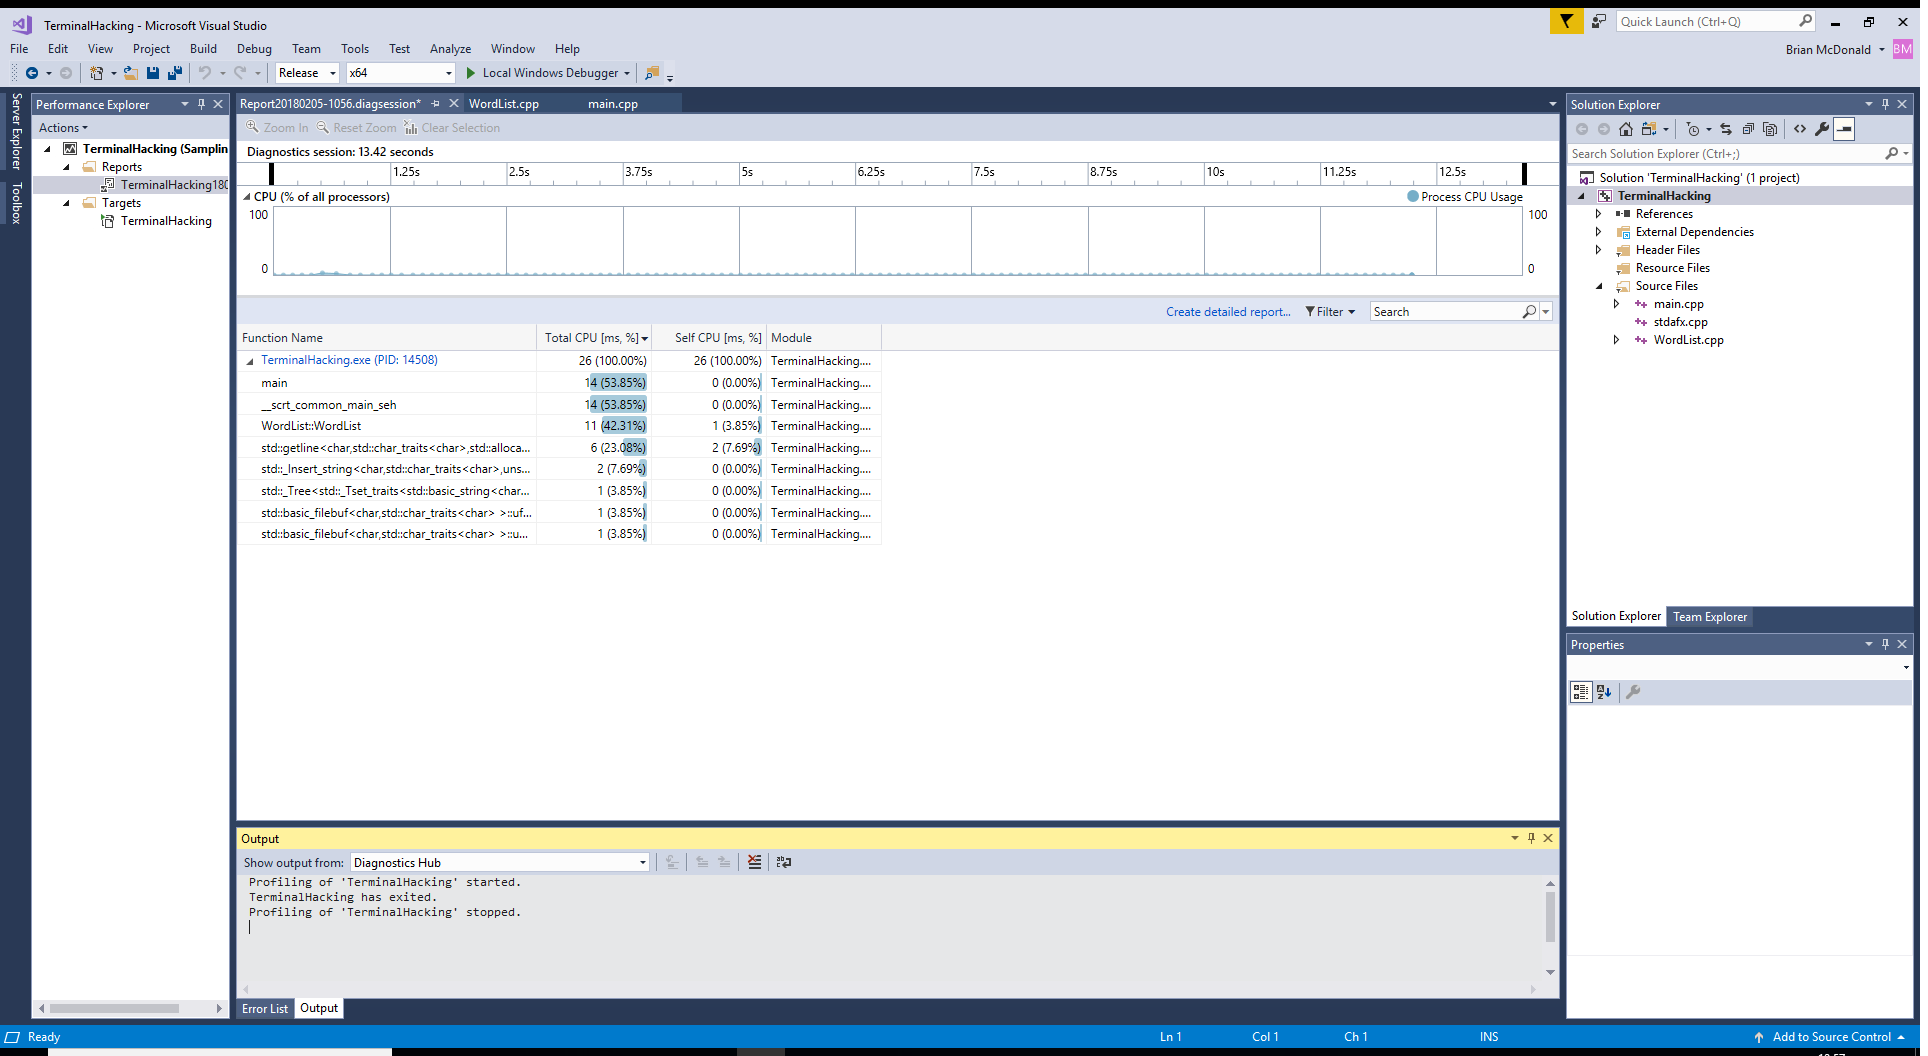
\includegraphics[width=\textwidth,height=\textheight,keepaspectratio]{VSProfilerWindow}
	\end{center}
\end{frame}


\begin{frame}{NVidia NSight}
	\begin{center}
		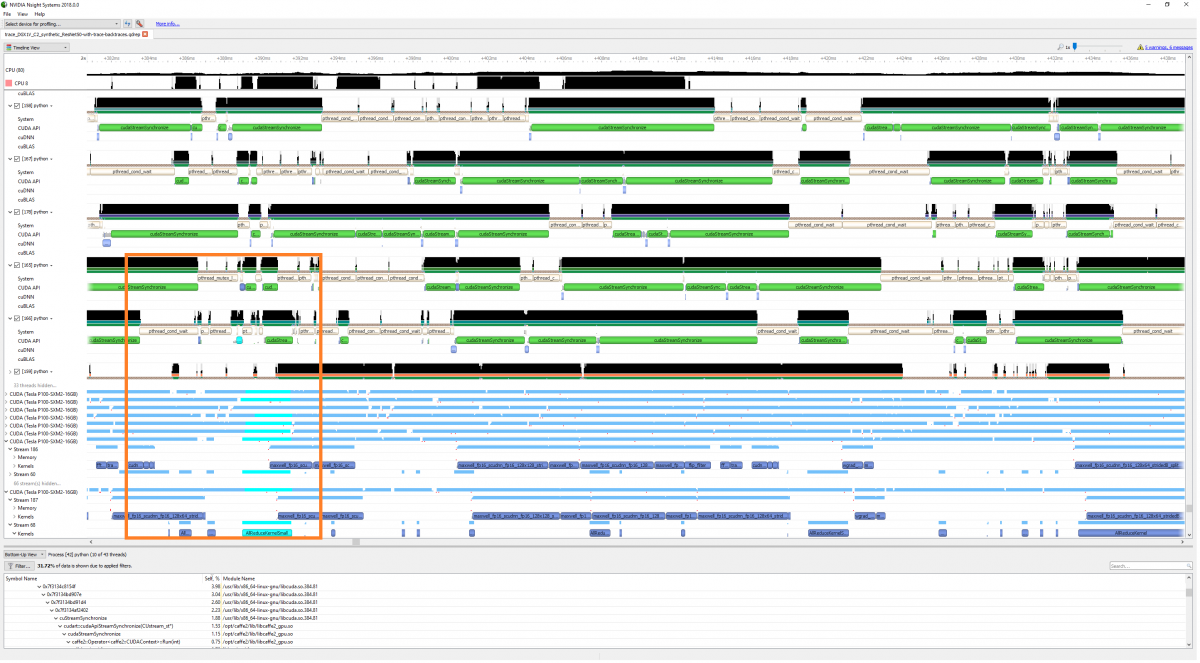
\includegraphics[width=\textwidth,height=\textheight,keepaspectratio]{n_sight}
	\end{center}
\end{frame}

\begin{frame}{Render Doc}
	\begin{center}
		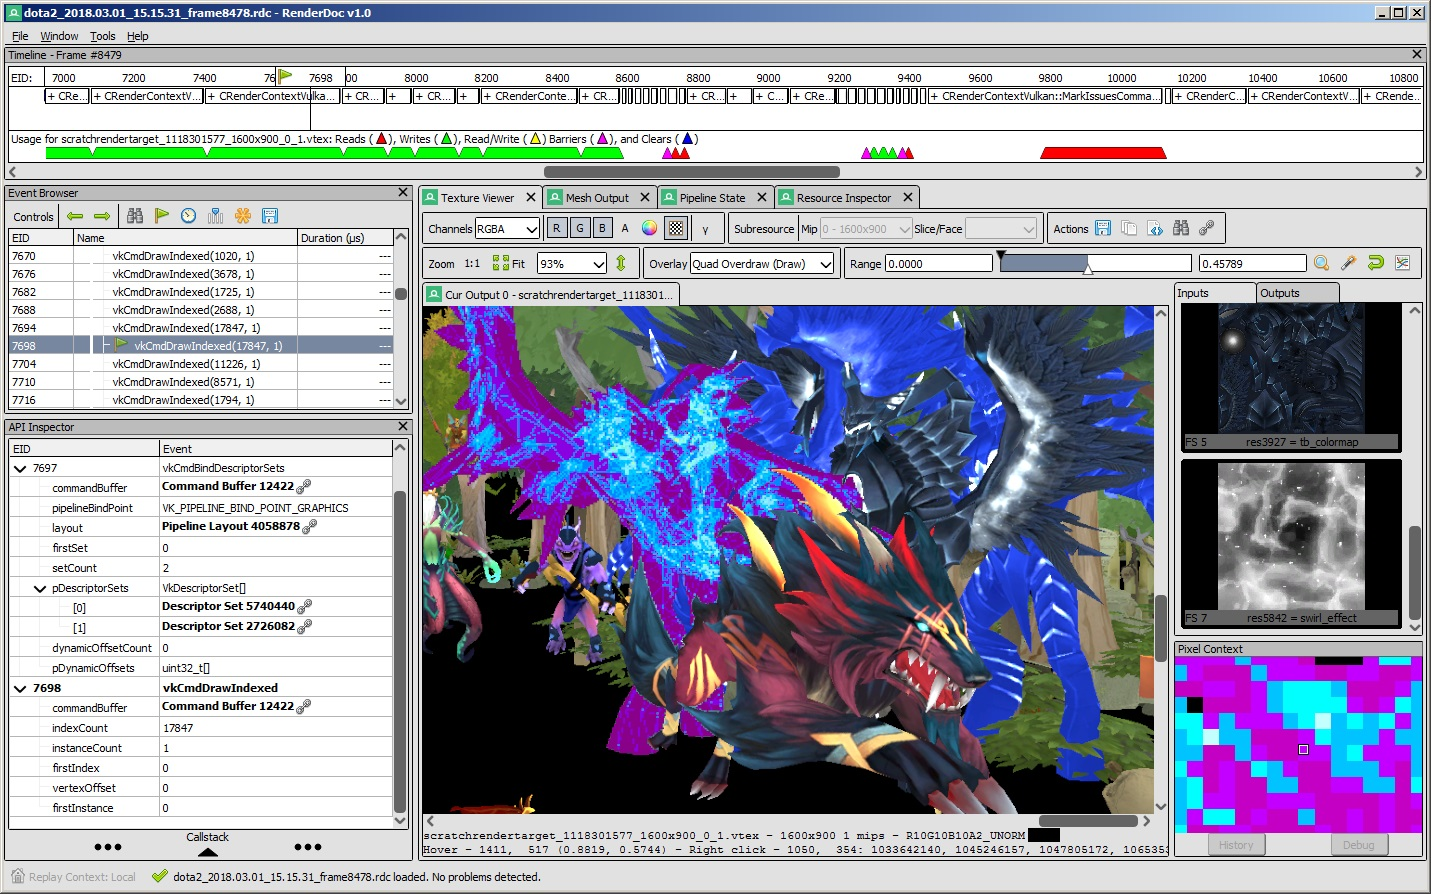
\includegraphics[width=\textwidth,height=\textheight,keepaspectratio]{render_doc}
	\end{center}
\end{frame}
\part{Worksheet}
\frame{\partpage}

\begin{frame}{Optimisation Worksheet}
	\url{https://learningspace.falmouth.ac.uk/mod/resource/view.php?id=114234}
\end{frame}

\frame{\partpage}

\end{document}
